\section{User Interface Results}
This section illustrates the core functionality of AyurSpace from the user's perspective,
highlighting the UI rendering of state changes managed by Flutter and Riverpod.

\begin{figure}[!htbp]
    \centering
    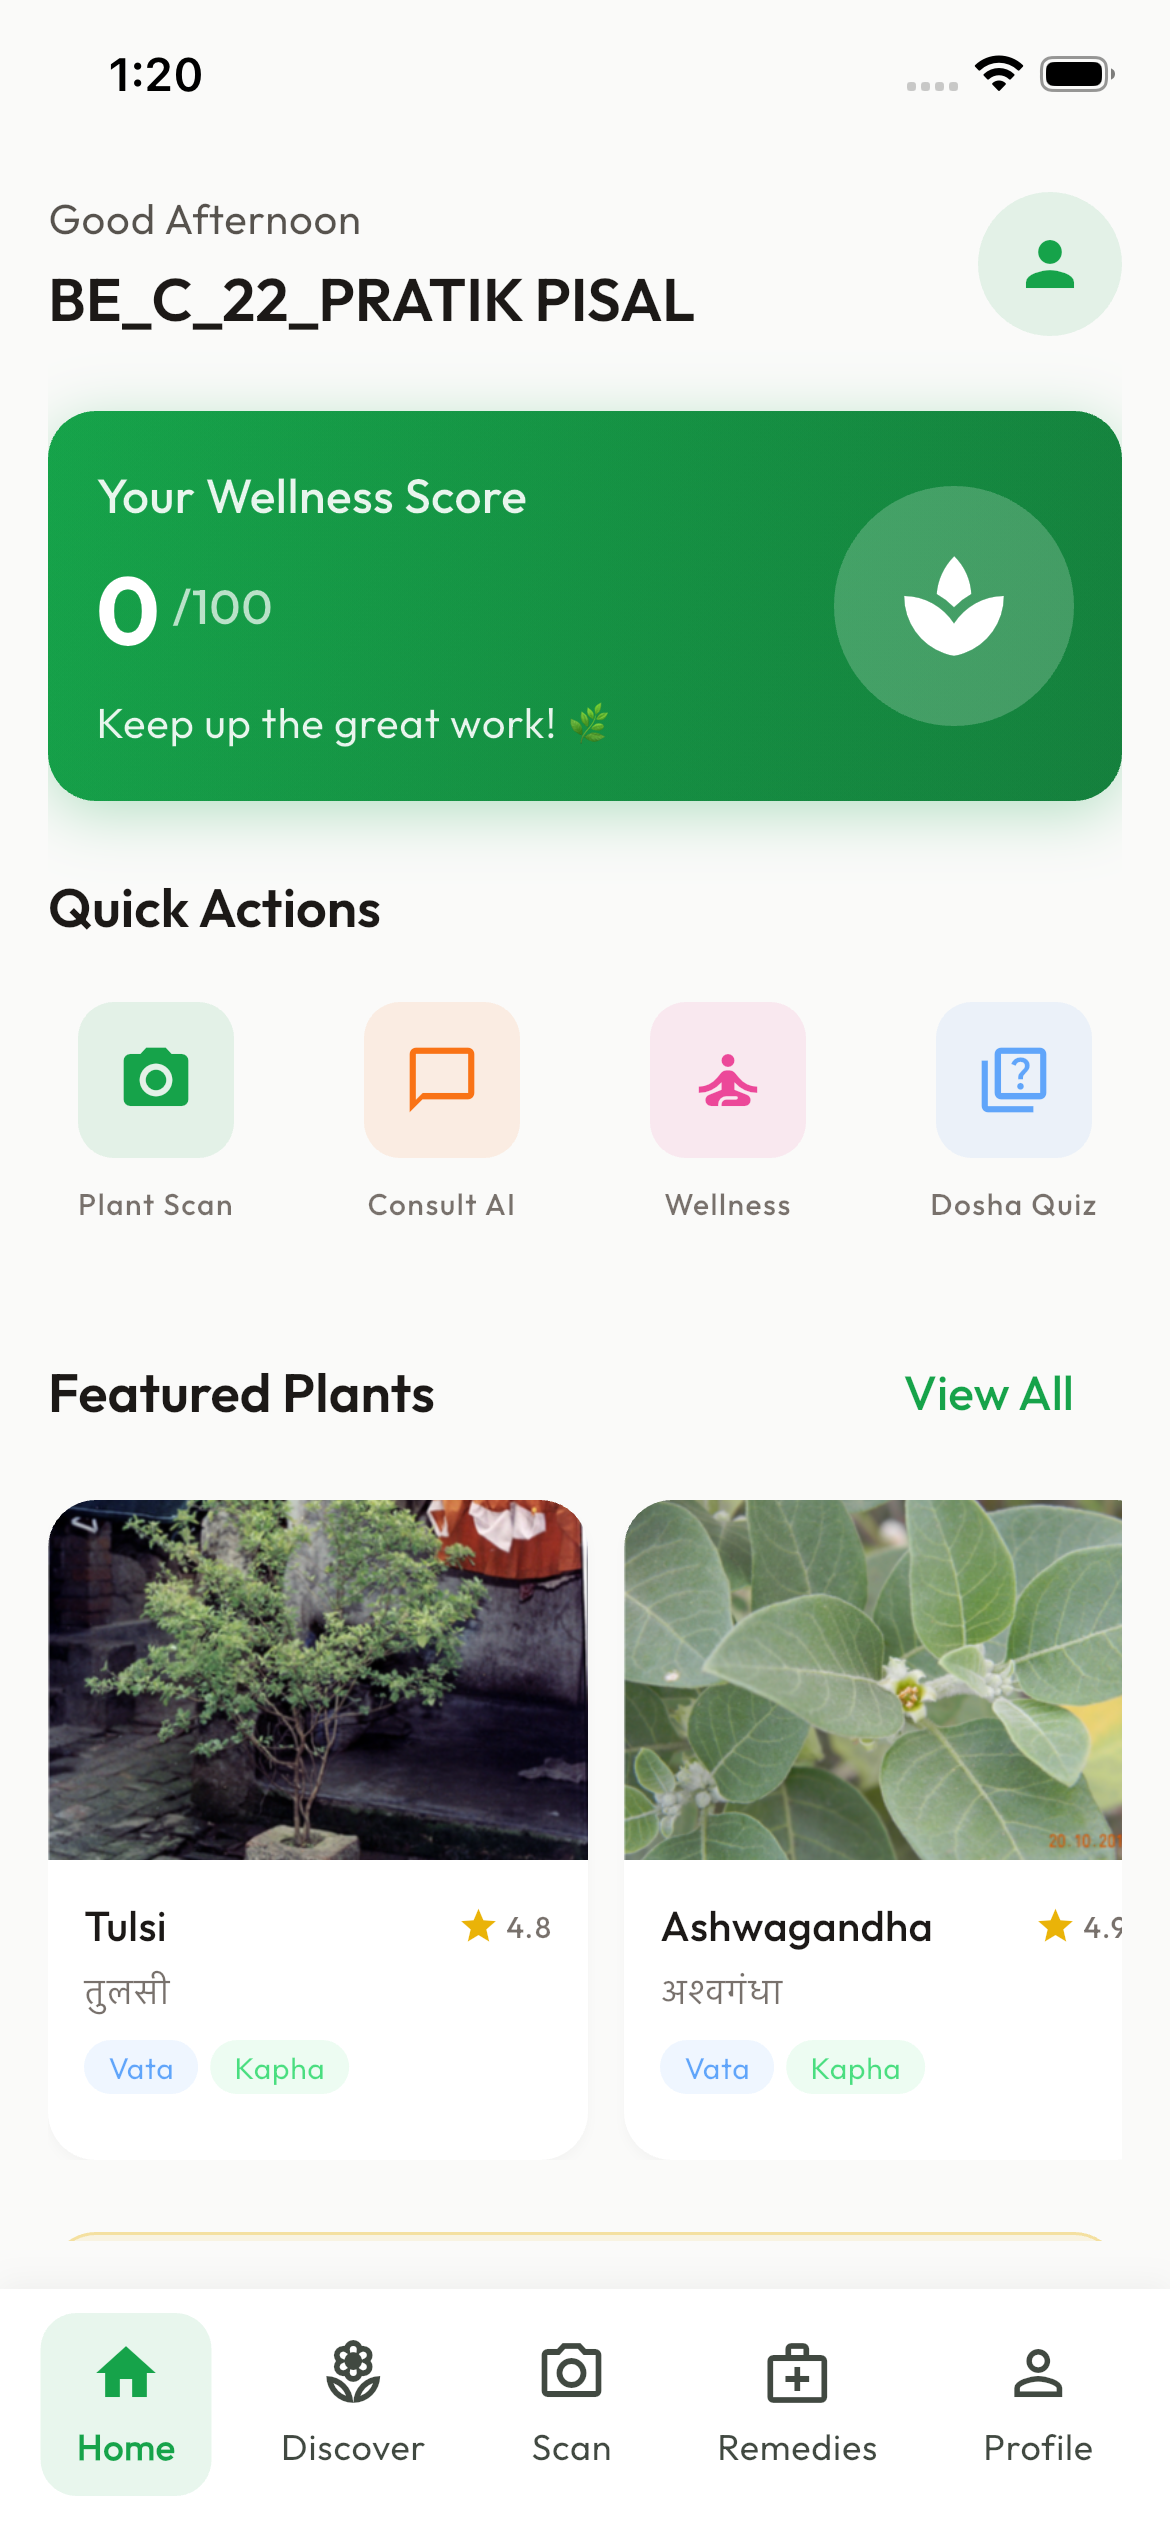
\includegraphics[width=0.3\textwidth]{assets/screenshots/home_screen.png}
    \caption{AyurSpace Home Dashboard}
    \vspace{10pt}
    \justify
    The Home Dashboard is the orchestration hub for plant scanning,
    dosha assessments, and personalized wellness charts synchronized via Cloud Firestore.
\end{figure}

\newpage
\begin{figure}[!htbp]
    \centering
    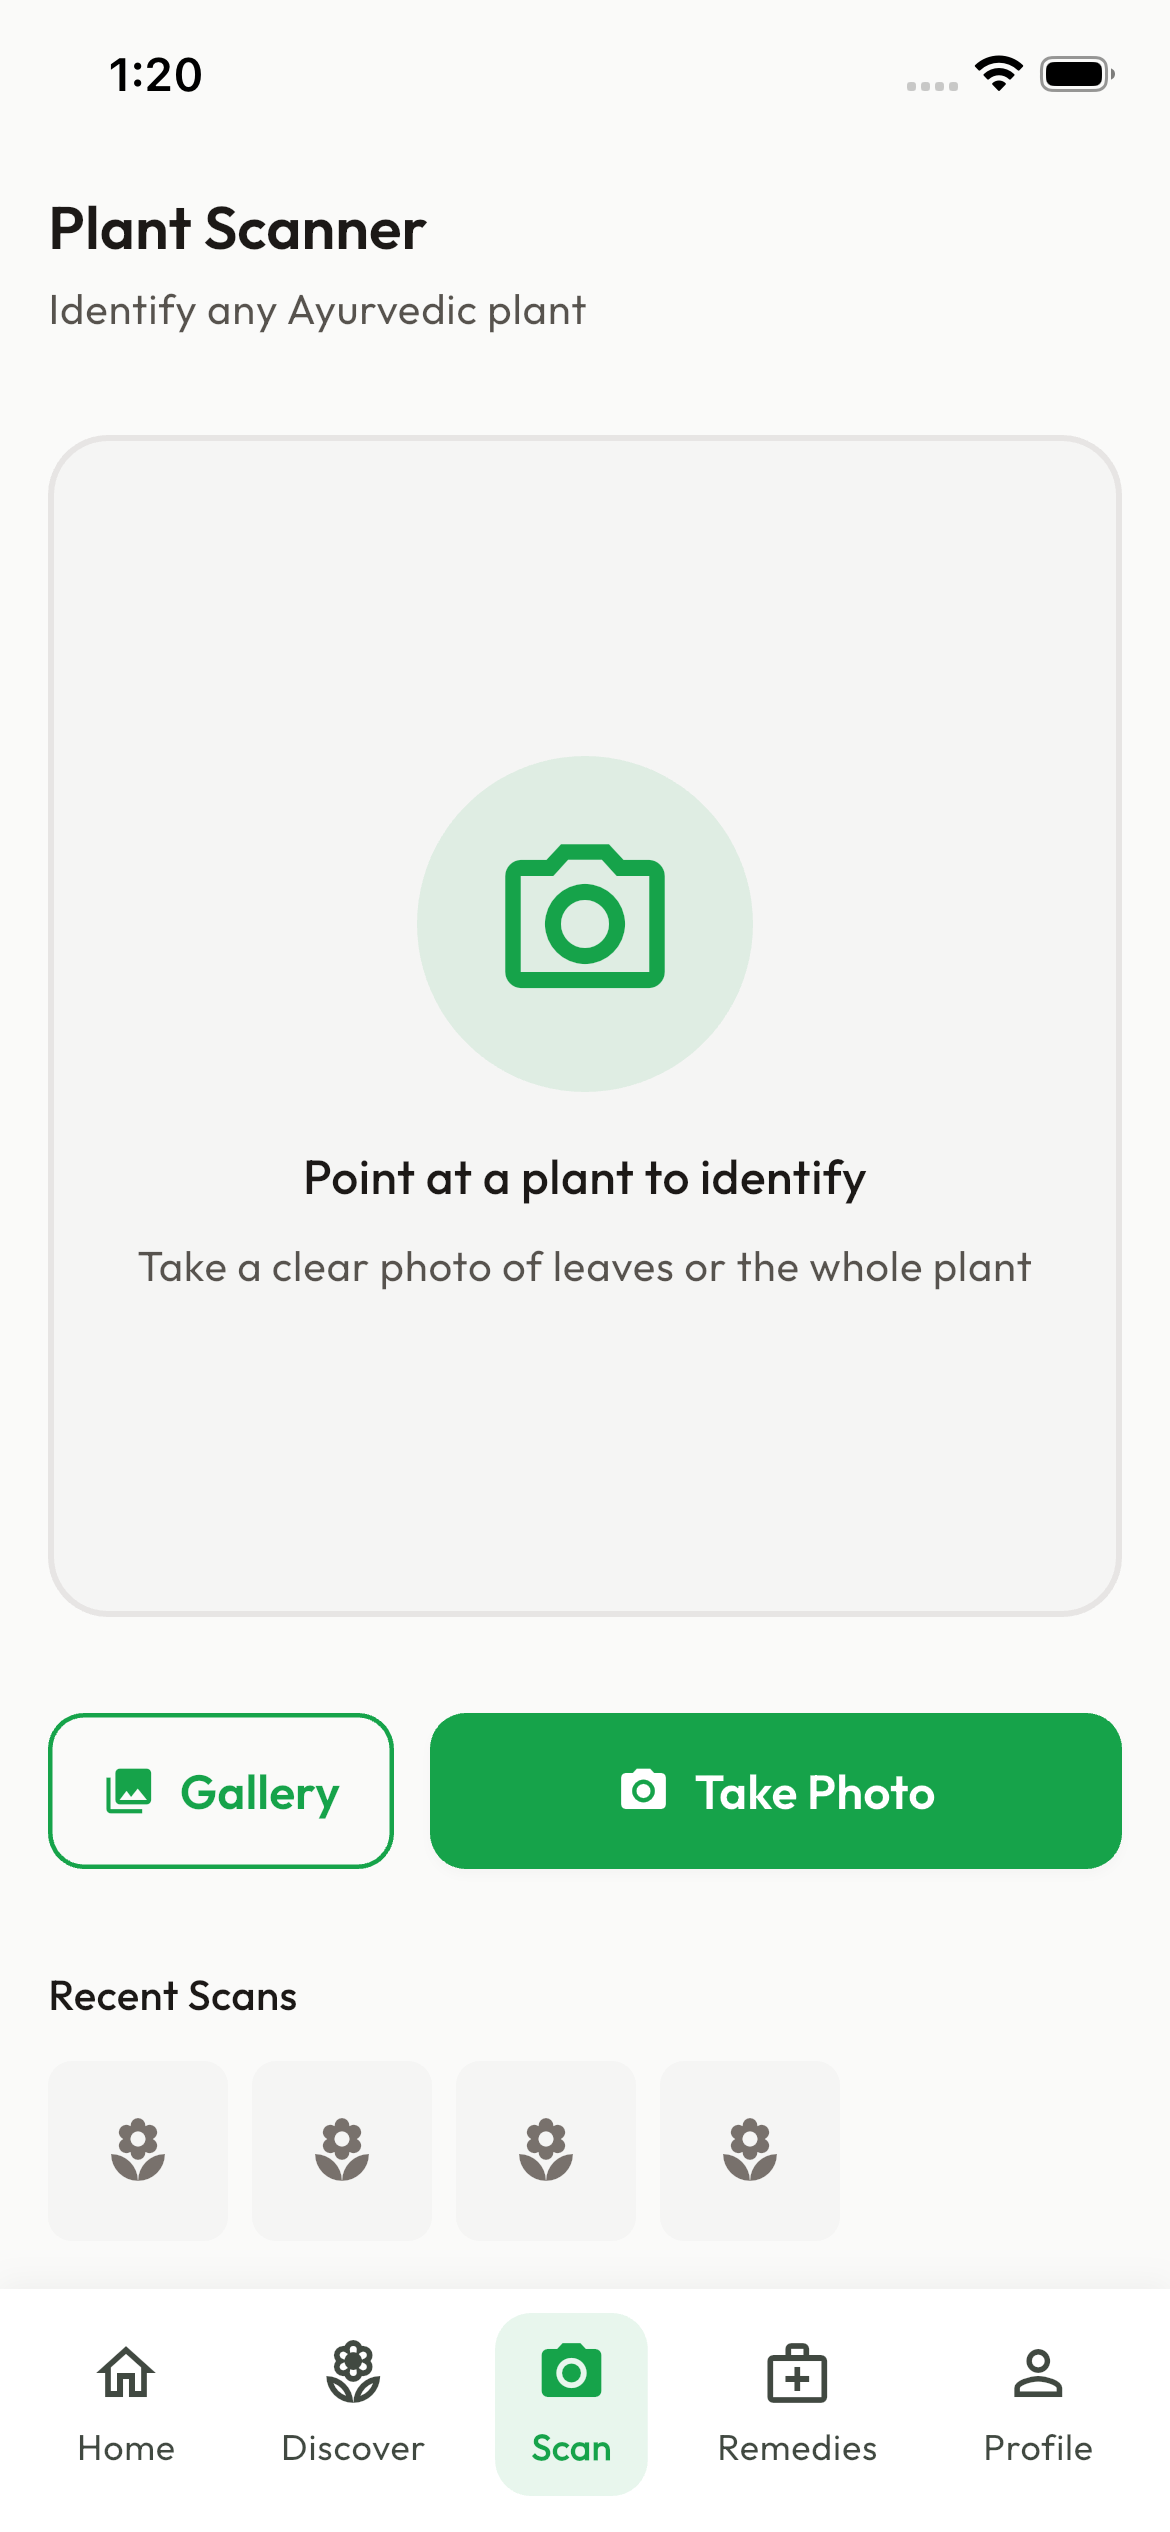
\includegraphics[width=0.3\textwidth]{assets/screenshots/scan_plant_screen.png}
    \caption{Plant Scanning Interface}
    \vspace{10pt}
    \justify
    The Plant Scanning Interface. The captured image undergoes
    $P(I_{raw})$ downsampling before being dispatched to Plant.id over HTTP.
\end{figure}

\begin{figure}[!htbp]
    \centering
    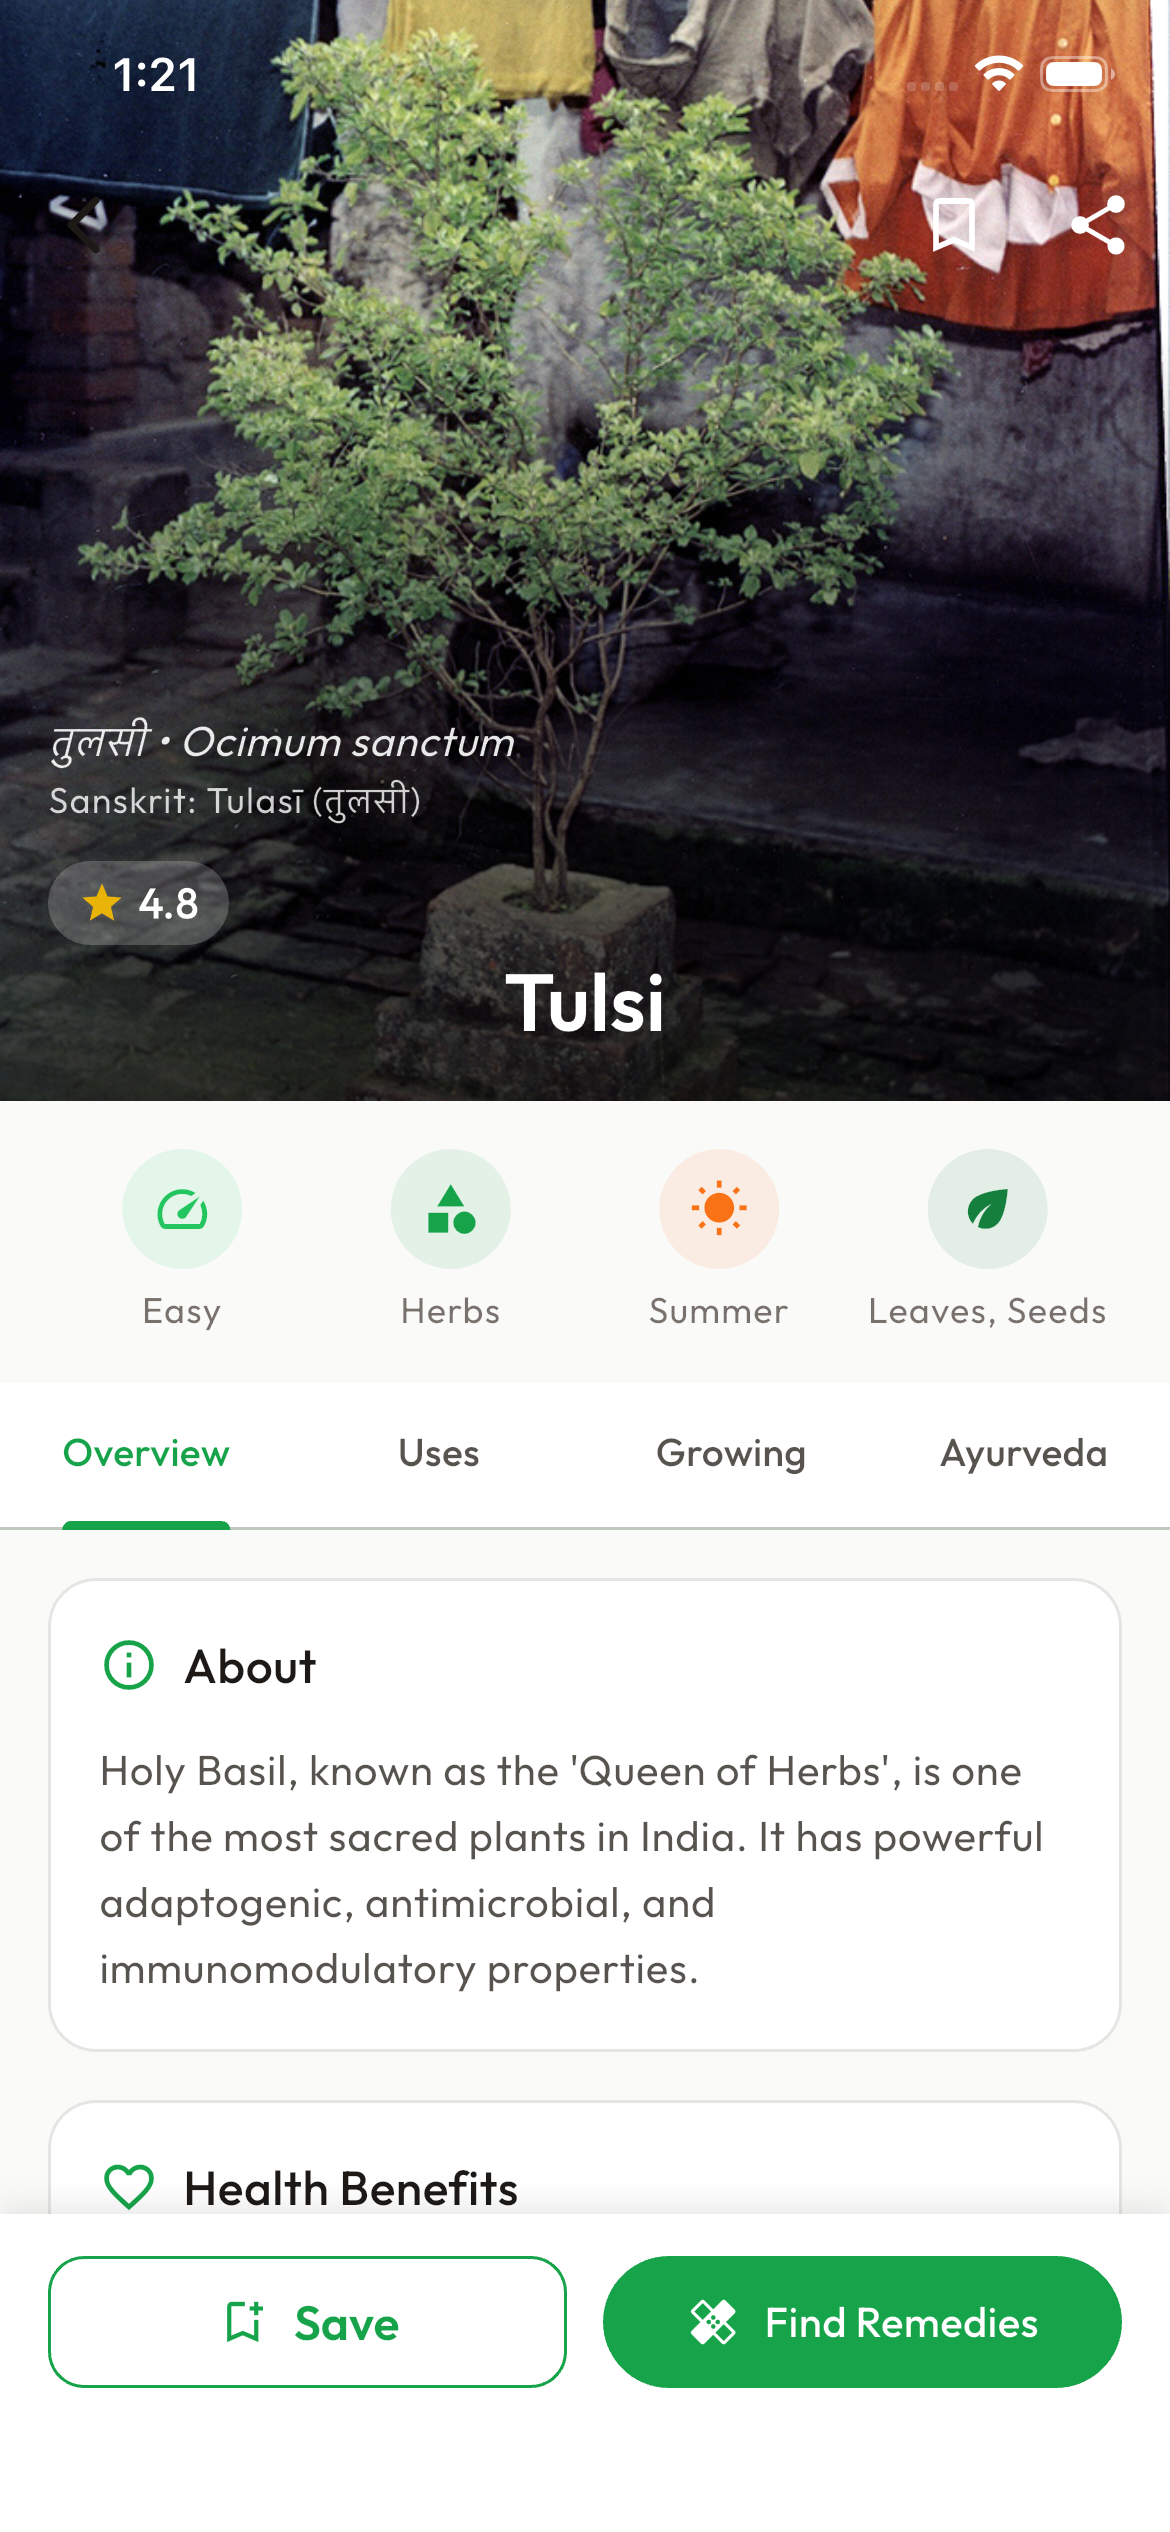
\includegraphics[width=0.3\textwidth]{assets/screenshots/plant_detail_screen.png}
    \caption{AI Diagnostic Results and Plant Detail}
    \vspace{10pt}
    \justify
    Fused output from Plant.id taxonomy + Gemini LLM contextual
    \textit{Rasa, Guna, Virya, Vipaka} data.
\end{figure}

\begin{figure}[!htbp]
    \centering
    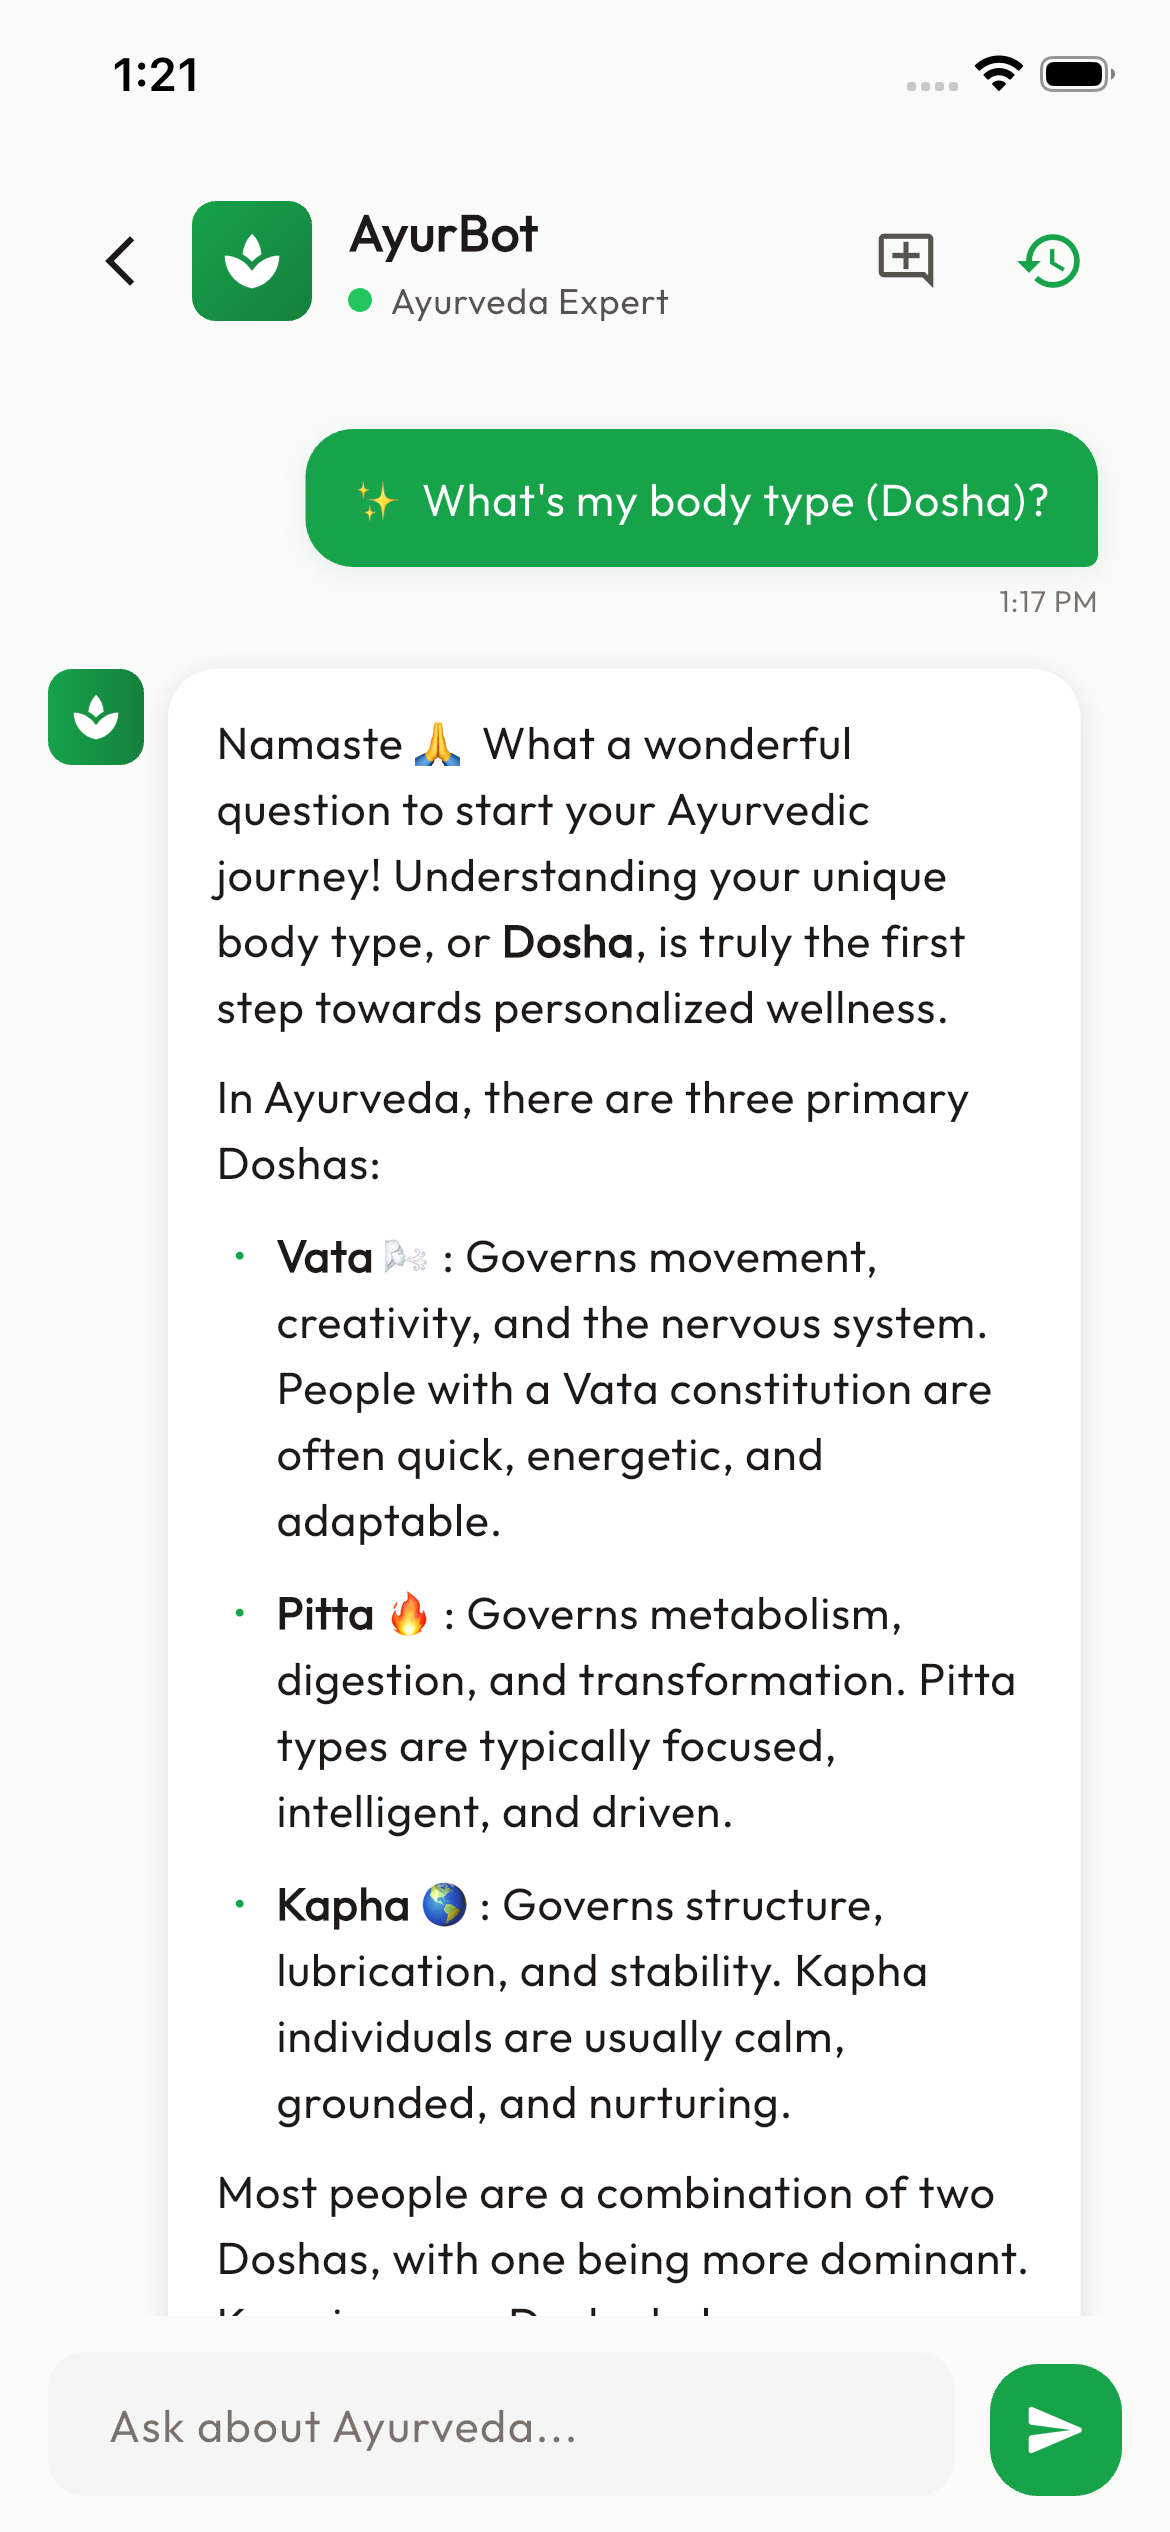
\includegraphics[width=0.3\textwidth]{assets/screenshots/AyurBot_screen.png}
    \caption{AyurBot Chat Session}
    \vspace{10pt}
    \justify
    Multi-turn AyurBot session. Riverpod \texttt{ChatNotifier} renders
    message bubbles while passing the dosha context silently via System Instruction API.
\end{figure}

\begin{figure}[!htbp]
    \centering
    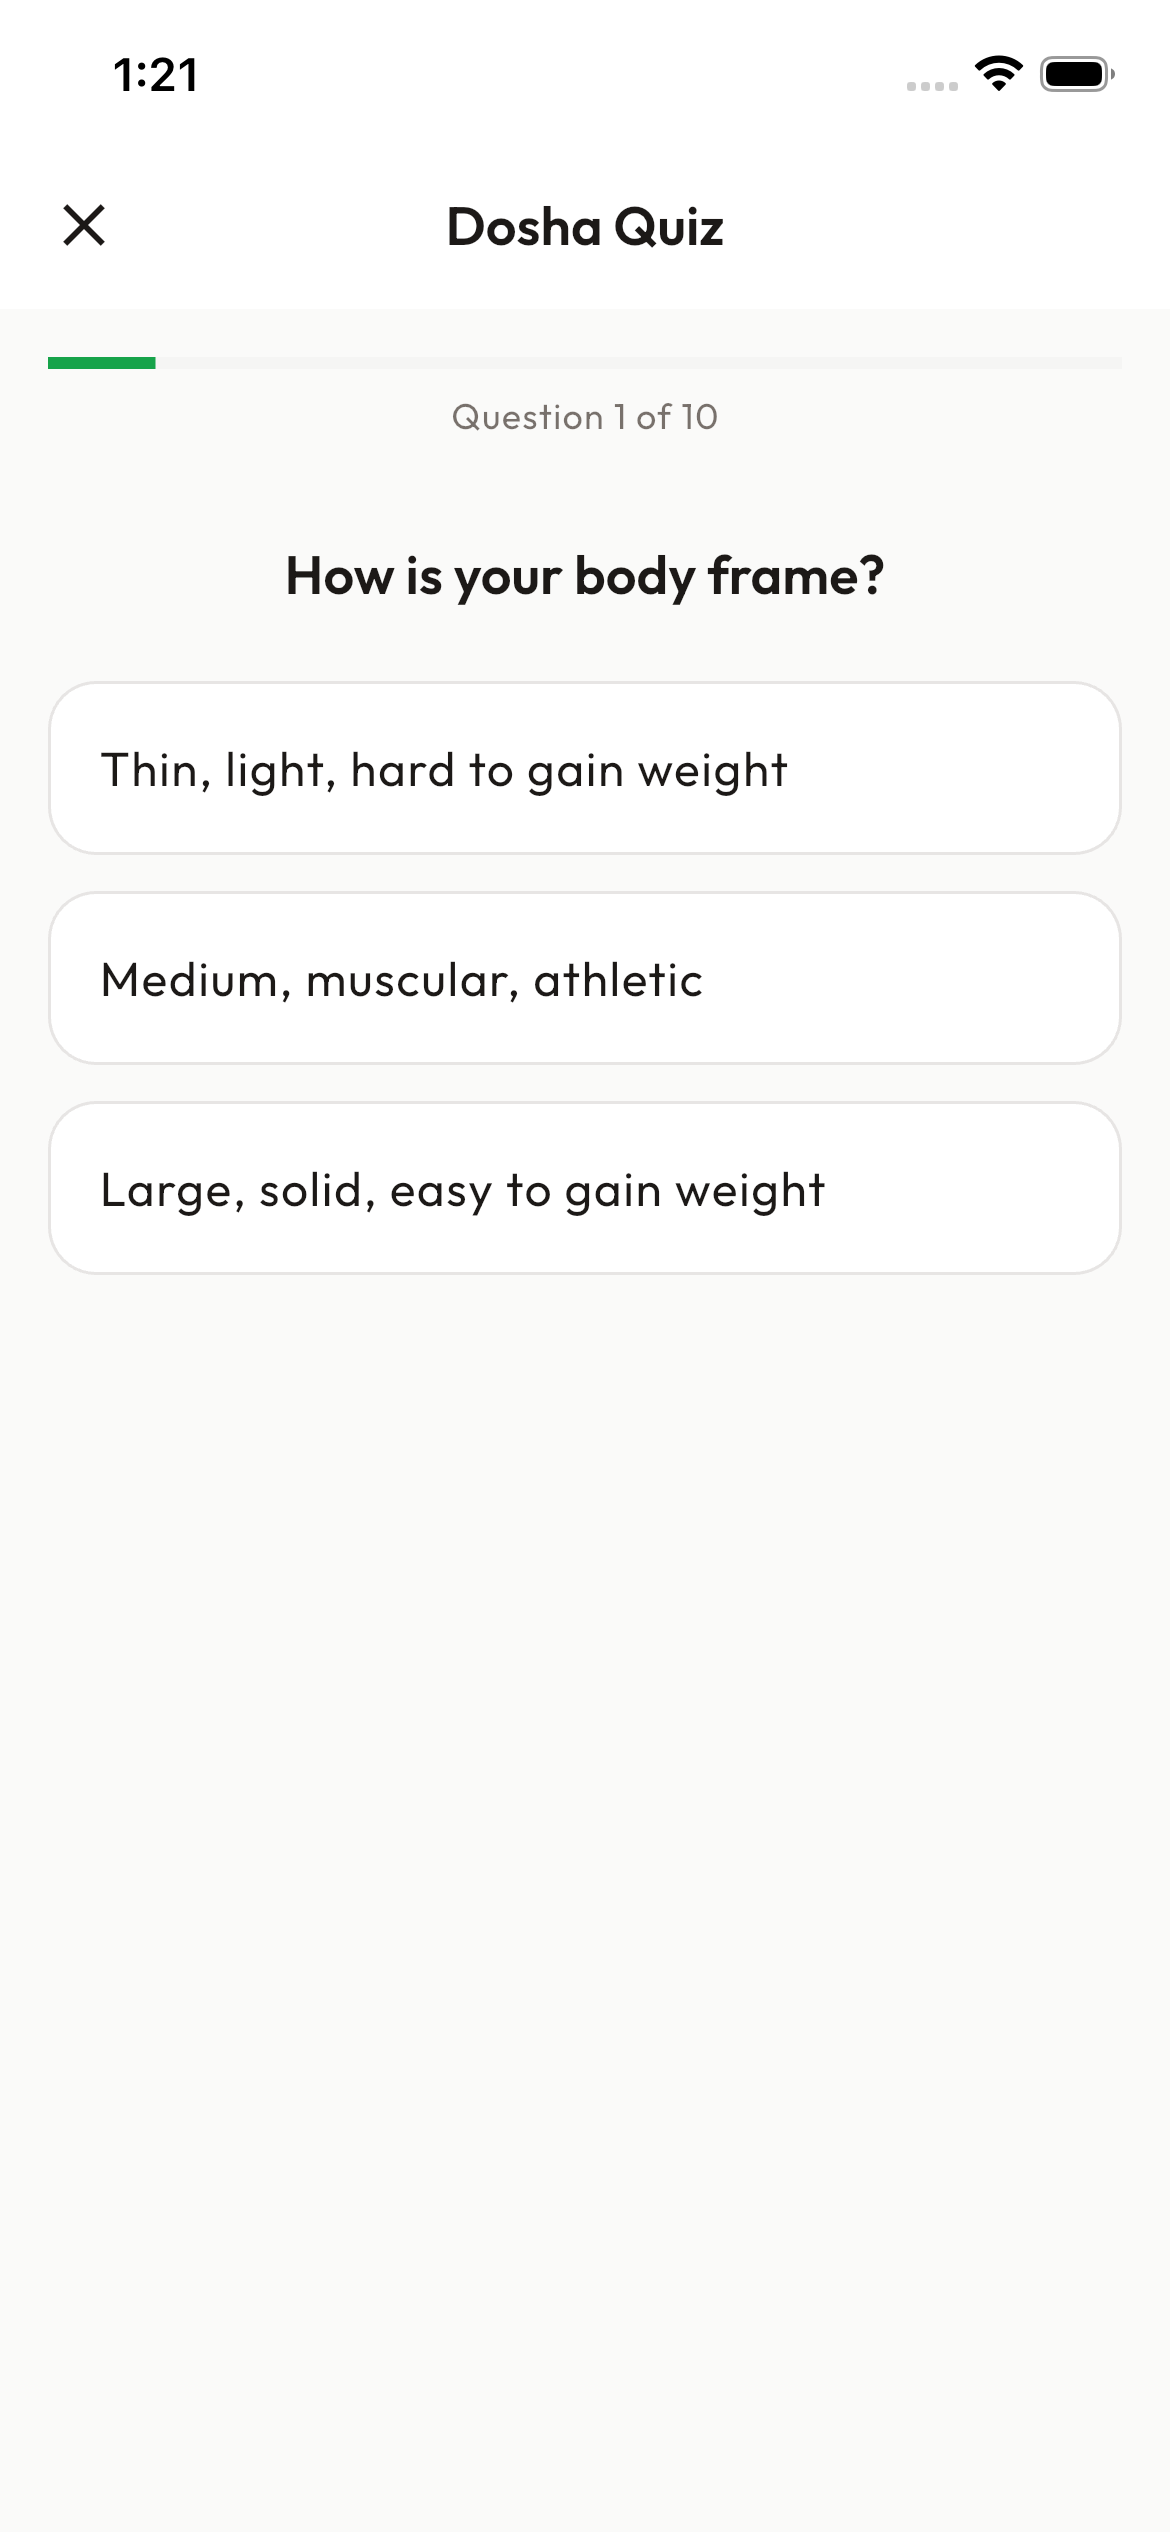
\includegraphics[width=0.3\textwidth]{assets/screenshots/dosha_quiz_screen.png}
    \caption{Tridosha Quiz Assessment Screen}
    \vspace{10pt}
    \justify
    The Tridosha Quiz. User choices are bound to algorithmic weights,
    resolving into a discrete mathematical model for baseline health prediction.
\end{figure}

\newpage
\section{Experimental Setup \& Metric Definition}
\begin{enumerate}
    \item \textbf{Top-1 Identification Accuracy ($Acc_1$)}: Frequency of correct species
    as the first suggestion returned.
    \item \textbf{Hallucination Rate ($H_r$)}: Frequency of incorrect LLM-generated plant
    properties.
    \item \textbf{End-to-End Latency ($L_{total}$)}: Full time from capture to last UI
    render.
\end{enumerate}
Testing performed on a mid-range Android device over 4G LTE. Dataset: 50 Indian medicinal
plant species (e.g., \textit{Ocimum sanctum, Azadirachta indica, Tinospora cordifolia}).

\section{Performance Benchmarks}
\begin{table}[htbp]
\caption{System Performance Benchmarks}
\begin{center}
\begin{tabular}{|c|c|l|}
\hline
\textbf{Metric} & \textbf{Value} & \textbf{Notes} \\
\hline
Plant.id Accuracy & 96.4\% & Precision on top-1 prediction \\
\hline
Gemini Conformance & 99.1\% & Valid JSON schema generation \\
\hline
Comp. Efficiency & 85\% & Payload cut to $\approx$850KB \\
\hline
Avg. ID Latency & 2.1s & Plant.id API response time \\
\hline
Avg. LLM Latency & 1.8s & Gemini 2.5 Flash inference \\
\hline
\textbf{Total Latency} & \textbf{4.2s} & End-to-end UX threshold \\
\hline
\end{tabular}
\end{center}
\end{table}

Total latency of 4.2s is acceptable for non-real-time educational apps. Compression adds
200ms overhead but saves $\approx$1.5s in network transfer compared to raw uploads.

\section{Ablation Study}
\begin{itemize}
    \item \textbf{Pathway A (Control)}: Direct image to Gemini Vision.\\
    Result: Inconsistent; occasional plant misidentification.
    \item \textbf{Pathway B (AyurSpace Hybrid)}: Plant.id + Gemini.\\
    Result: Accurate, medically correct, and structured output with confidence scores.
\end{itemize}
\textbf{Conclusion}: Specialized Narrow AI (Vision) + Generalized AI (Reasoning)
significantly outperforms Generalized Multi-modal AI alone.
